\section{Принципы и логическая модель решения}

Для реализации интеллектуального модуля интерактивного анализа данных была спроектирована распределенная микросервисная архитектура, основанная на парадигме RAG (Retrieval-Augmented Generation). Логическая модель системы строится на разделении процессов накопления знаний (Ingest Pipeline) и процессов генерации ответов на запросы пользователя (Retrieval Pipeline).

\subsection{Ключевые архитектурные принципы}

В основу проектируемого решения заложено несколько сквозных инженерных принципов. Прежде всего, это микросервисная организация, при которой каждый функциональный блок — векторизация, поиск, работа с базой данных — вынесен в отдельный сервис. Такой подход позволяет независимо масштабировать компоненты и использовать разные стеки технологий: например, GPU-зависимые сервисы для языковых моделей соседствуют с лёгковесными API для пользовательского интерфейса.

Далее, система строится на принципе слабой связанности (Loose Coupling). Взаимодействие между компонентами осуществляется строго через REST API, а прямой доступ к реляционной базе данных централизован через сервис-прослойку \texttt{db\_connector\_service}. Это исключает конфликты транзакций и заметно упрощает возможную смену СУБД в будущем.

Важную роль играет асинхронность и реактивность. Длительные операции — такие как парсинг схем данных или векторизация больших документов — выполняются в фоновом режиме с использованием очередей задач на базе Redis. Наконец, в системе реализовано разделение конвейеров данных: процессы индексации знаний и обработки текущих запросов изолированы друг от друга, что обеспечивает высокую доступность даже в моменты обновления базы знаний.

\subsection{Описание компонентов системы (HLD)}

Cистема включает в себя несколько ключевых сервисов. Пользовательский интерфейс, построенный на Gradio или веб-технологиях, служит точкой входа: именно здесь происходит визуализация результатов анализа и управление диалогом. За логику рассуждения отвечает модуль агента (Agent Module), который реализует паттерн Chain-of-Thought. Агент принимает решение, требуется ли простое обращение к базе данных или необходимо задействовать RAG-конвейер для извлечения дополнительного контекста о структуре БД. Центральным оркестратором выступает RAG Service, который объединяет результаты поиска из векторного хранилища ChromaDB с промптом для языковой модели. Наконец, Embedding Model Service представляет собой локальный сервис на базе моделей HuggingFace, отвечающий за преобразование текстовых данных в многомерные векторы-эмбеддинги. Общая HLD-диаграмма системы представлена на рисунке \ref{fig:hld}.

\begin{figure}[H]
    \centering
    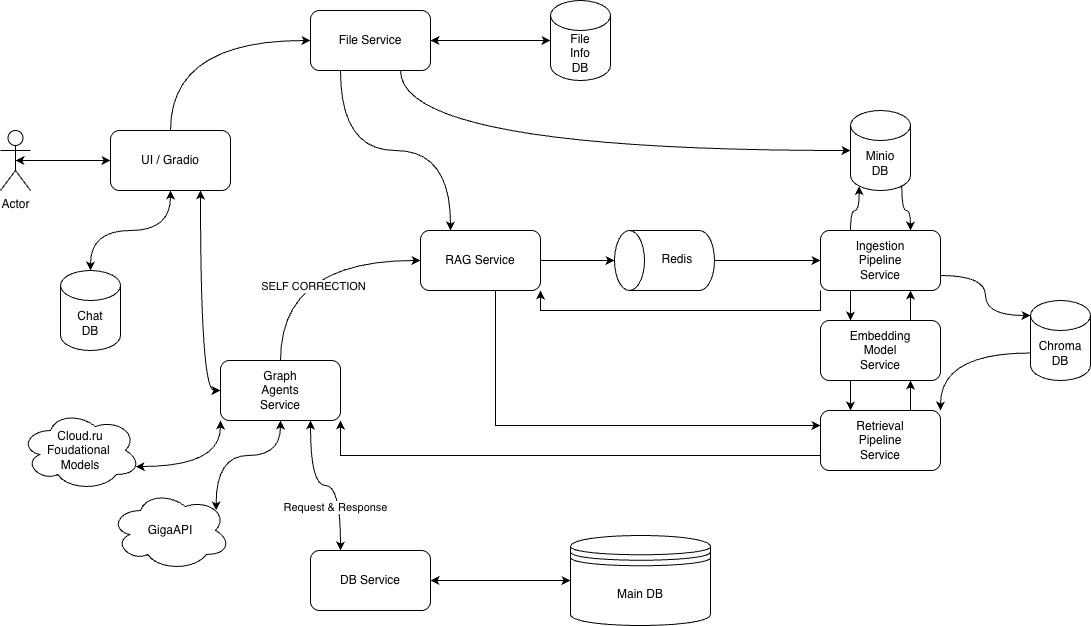
\includegraphics[width=0.9\textwidth]{materials/HLD.drawio.png}
    \caption{HLD диаграмма системы}
    \label{fig:hld}
\end{figure}

\subsection{Логика работы конвейера обработки данных (RAG Pipeline)}

Процесс работы модуля можно разделить на два независимых цикла, которые хорошо видны на схеме RAG Pipeline. Первый из них — цикл индексации (Ingest). На этом этапе исходные данные, включая документацию к базе данных, схемы таблиц Postgres Pro и описание предметной области авиаперевозок, сохраняются в хранилище MinIO, разбиваются на фрагменты (чанки) и индексируются в ChromaDB. Второй цикл — цикл генерации (Retrieval) — запускается уже во время работы с пользователем. Когда от пользователя поступает вопрос, например «Покажи загрузку рейсов из Шереметьево», система векторизует запрос, находит в хранилище релевантные описания таблиц и передаёт их в языковую модель для генерации корректного SQL-запроса.

Схема работы RAG Pipeline приведена на рисунке \ref{fig:ragpipeline}.

\begin{figure}[H]
    \centering
    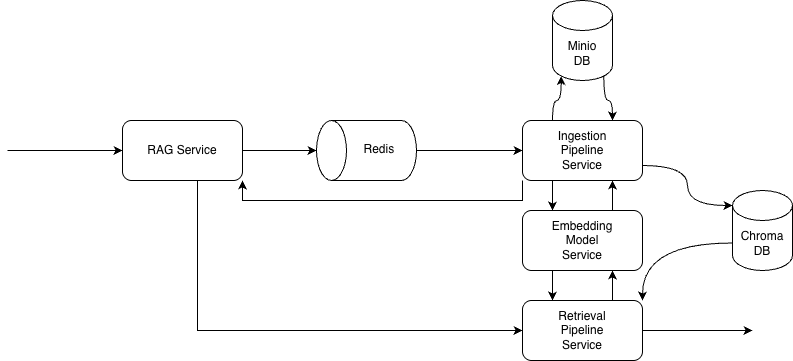
\includegraphics[width=0.9\textwidth]{materials/rag_pipeline.drawio.png}
    \caption{Архитектурная реализация RAG Pipeline}
    \label{fig:ragpipeline}
\end{figure}

Диаграмма последовательности действий системы при обработке запроса пользователя представлена на рисунке \ref{fig:userflow}.

\begin{figure}[H]
    \centering
    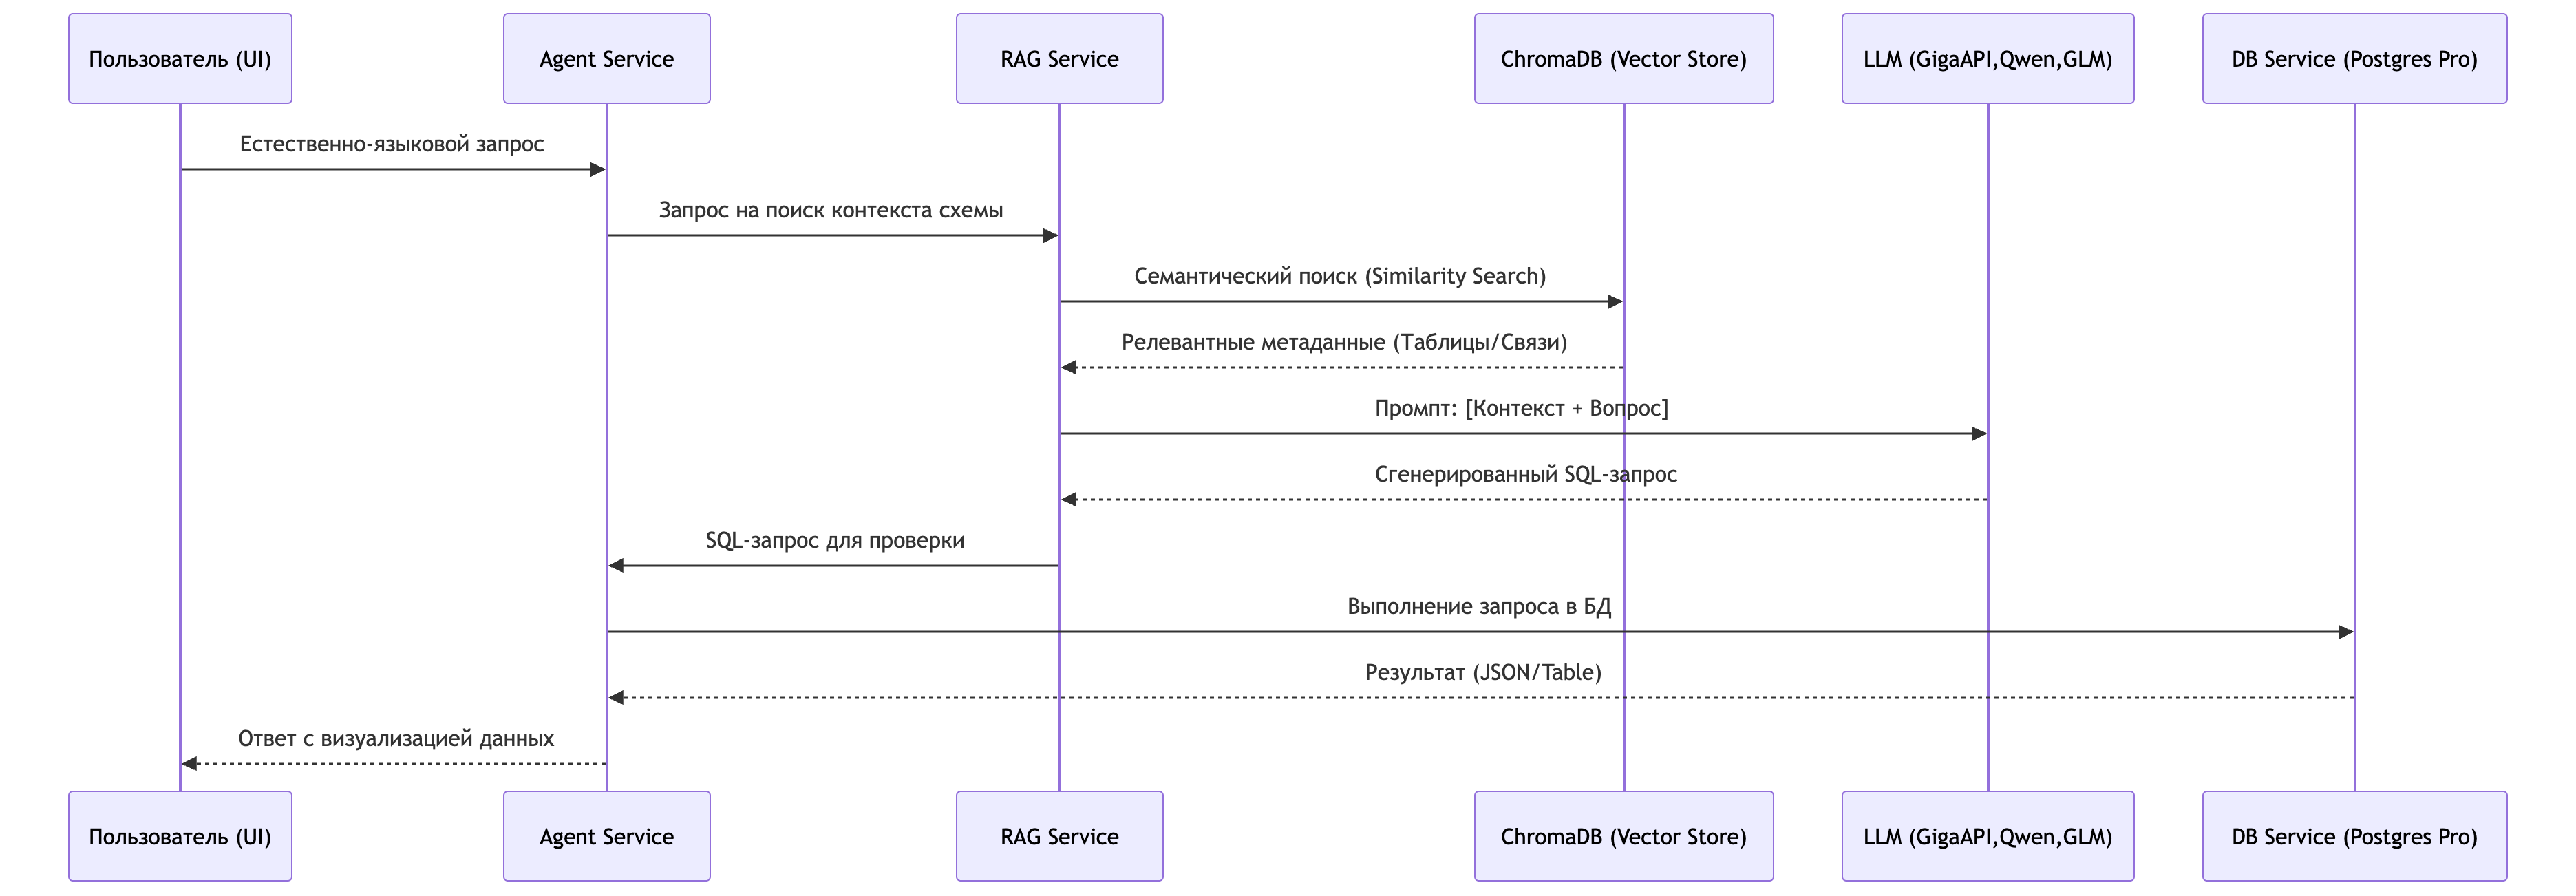
\includegraphics[width=0.9\textwidth]{materials/user_flow.png}
    \caption{Сценарий использования пользователем системы (UserFlow)}
    \label{fig:userflow}
\end{figure}


\subsection{Принцип самокоррекции (Self-Heal)}

Особенностью логической модели является наличие обратной связи в агентском сервисе. Если при выполнении сгенерированного SQL-запроса СУБД возвращает ошибку (например, неверный синтаксис или отсутствие столбца), агент перехватывает исключение и инициирует повторный цикл генерации, передавая текст ошибки обратно в LLM. Это позволяет достичь высокой надежности системы в условиях работы со сложными схемами данных, такими как база «Авиаперевозки» от Postgres Pro. Блок-схема механизма самокоррекции приведена на рисунке \ref{fig:selfcorrection}.

\begin{figure}[H]         
    \centering             
    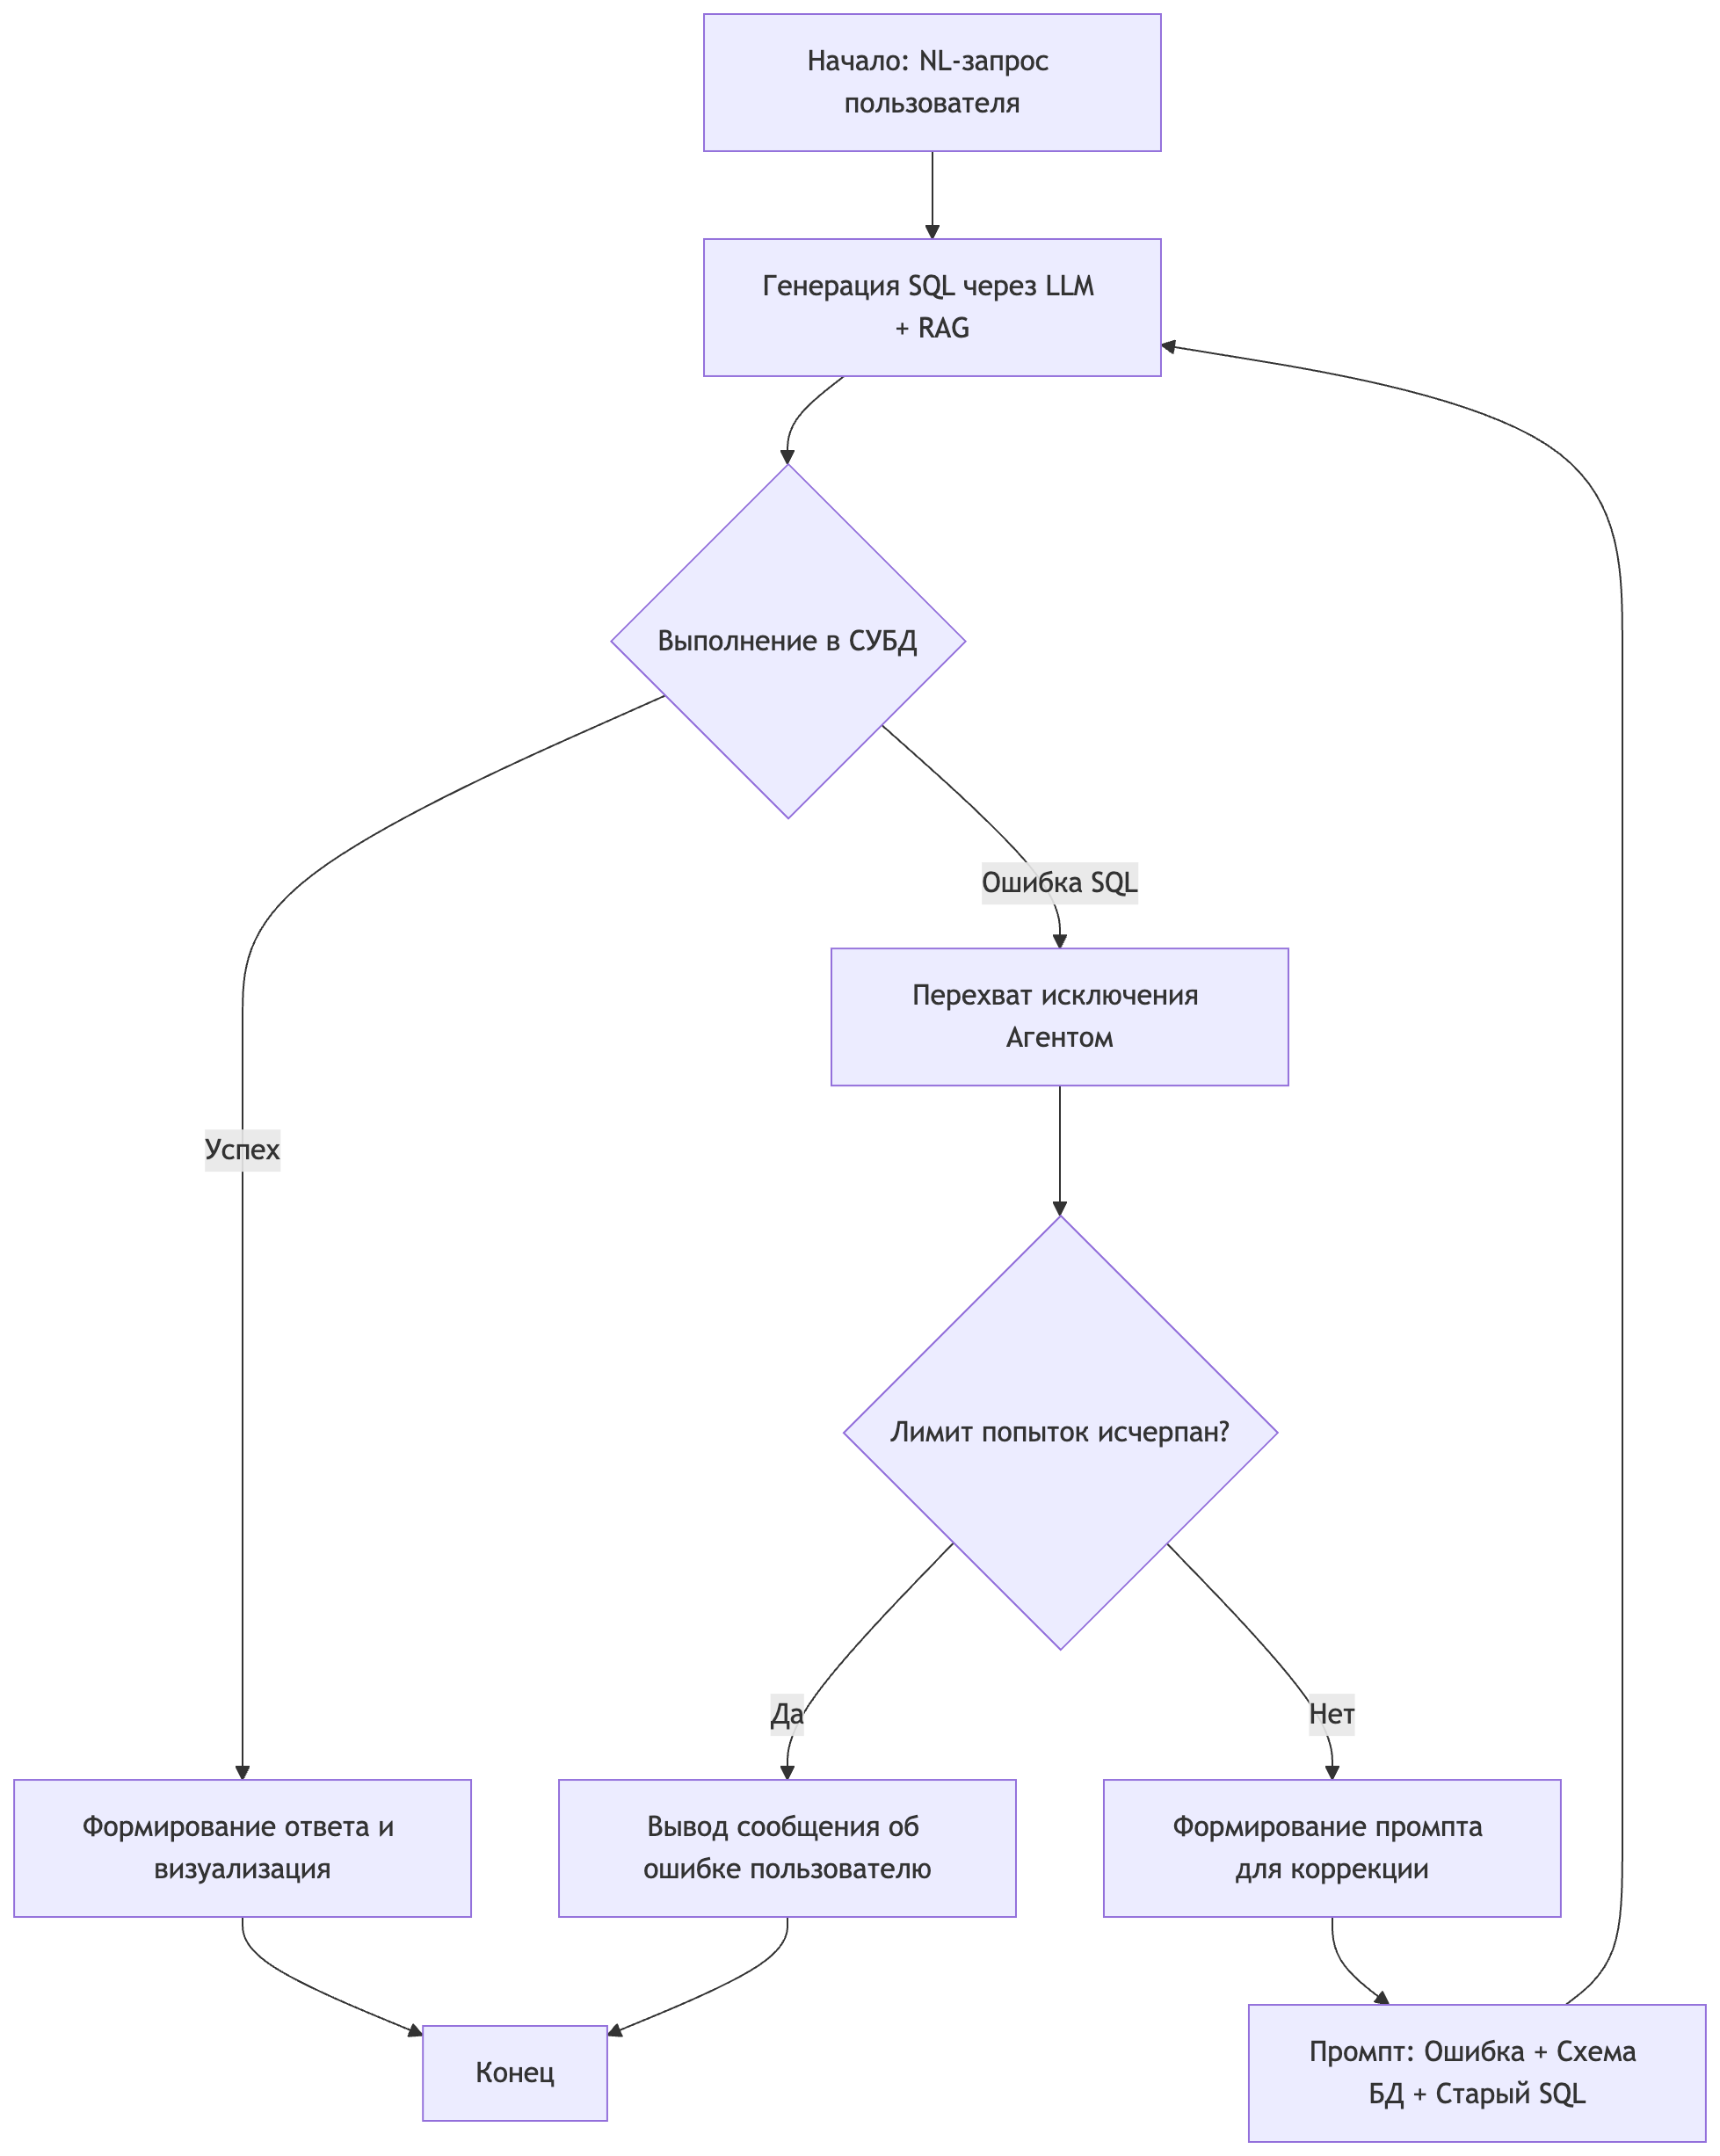
\includegraphics[width=0.65\textwidth]{materials/self_correction.png} 
    \caption{Блок схема механизма самокоррекции}
    \label{fig:selfcorrection}
\end{figure}
